% Chapter 3

\chapter{Test Specification} % Main chapter title

\label{Chapter3} % For referencing the chapter elsewhere, use \ref{Chapter1} 

%----------------------------------------------------------------------------------------

% Define some commands to keep the formatting separated from the content 
%\newcommand{\keyword}[1]{\textbf{#1}}
%\newcommand{\tabhead}[1]{\textbf{#1}}
%\newcommand{\code}[1]{\texttt{#1}}
%\newcommand{\file}[1]{\texttt{\bfseries#1}}
%\newcommand{\option}[1]{\texttt{\itshape#1}}

%----------------------------------------------------------------------------------------

\section{Overview}
\paragraph The test specification explained in this chapter serve also as a driver for the application design and development. While in the previous chapter was described the data model of each one of the services that form the application, in this one the behavior of each component as well as its connections with other services are explained through a set of Gherkin based files scoped at different test levels. The intention is  to simulate a BDD process and thus the test design process is the following:

\begin{enumerate}
	\item For each test level, define a Gherkin file that describes a functionality
	\item That file is then reviewed by the related stakeholders
	\item The functionality that will make that test set to pass is implemented
\end{enumerate}

\paragraph Of course item 2 is not happening during the implementation of this Project but is good to mention it anyway as it is quite the essence of using Gherkin language for test specification. The using of plain English files for describing how an application works should allow any stakeholder to participate openly in the way software is designed achieving greater team integration, improving communication and reducing misunderstandings to a minimum. Although its difficult to reflect the simulation of the BDD process in this document, the author will try to go through items 1 and 3 of the process in order to get an introduction as reliable as possible of an actual BDD process.

%\paragraph The reason behind using the process listed above is actually to compare previous test design strategies used by the author with this approach in a more complex application than the one used in the course. So the decision of using BDD instead of other strategies is just the auto imposed constraint of including it as one of the Project objectives and not the result of a comparison between different strategies.


%----------------------------------------------------------------------------------------

\section{Features}
\paragraph From the functional point of view, there have been defined two test levels for covering the major part of the use cases for the application:

\begin{itemize}
\item Integration Level: covers test cases coming from the integration of the Web Service and each one of the other services.
\item System Level: covers test cases that need the whole system to work. This is, use cases where interaction with different services is needed.
\end{itemize}

\paragraph From the non functional point of view, only test cases regarding availability have been considered. Test cases here involve the Discovery service and its ability to manage instances of the functional services.

\paragraph The following sub sections have been named after the feature file names, and in it is auto included the test type (either functional or non functional), the test level (either integration or system level), the service involved, and the test case number.

\subsection{functional-it-accountservice-1}
\ttfamily
\begingroup
\obeylines
\input{./../../sqa-project/features/functional-it-accountservice-1.feature}%
\endgroup%

\subsection{functional-it-accountservice-2}
\begingroup
\obeylines
\input{./../../sqa-project/features/functional-it-accountservice-2.feature}%
\endgroup%

\subsection{functional-it-accountservice-3}
\begingroup
\obeylines
\input{./../../sqa-project/features/functional-it-accountservice-3.feature}%
\endgroup%

\subsection{functional-it-productservice-1}
\begingroup
\obeylines
\input{./../../sqa-project/features/functional-it-productservice-1.feature}%
\endgroup%

\subsection{functional-it-orderservice-1}
\begingroup
\obeylines
\input{./../../sqa-project/features/functional-it-orderservice-1.feature}%
\endgroup%

\subsection{functional-it-cartservice-1}
\begingroup
\obeylines
\input{./../../sqa-project/features/functional-it-cartservice-1.feature}%
\endgroup%

\subsection{functional-st-1}
\begingroup
\obeylines
\input{./../../sqa-project/features/functional-st-1.feature}%
\endgroup%

\subsection{functional-st-2}
\begingroup
\obeylines
\input{./../../sqa-project/features/functional-st-2.feature}%
\endgroup%

\subsection{nonfunctional-availability-accounts}
\begingroup
\obeylines
\input{./../../sqa-project/features/nonfunctional-availability-accounts.feature}%
\endgroup%

\subsection{nonfunctional-availability-product}
\begingroup
\obeylines
\input{./../../sqa-project/features/nonfunctional-availability-product.feature}%
\endgroup%

\subsection{nonfunctional-availability-cart}
\begingroup
\obeylines
\input{./../../sqa-project/features/nonfunctional-availability-cart.feature}%
\endgroup%

\subsection{nonfunctional-availability-order}
\begingroup
\obeylines
\input{./../../sqa-project/features/nonfunctional-availability-order.feature}%
\endgroup%
\normalfont

\section{Class Diagram}
\paragraph After describing the application requirements in the previous sub chapters, the main relationships and dependencies between services are set. The diagram \ref{fig:Class Diagram} shows those dependencies.

\begin{figure}[!htb]
\centering
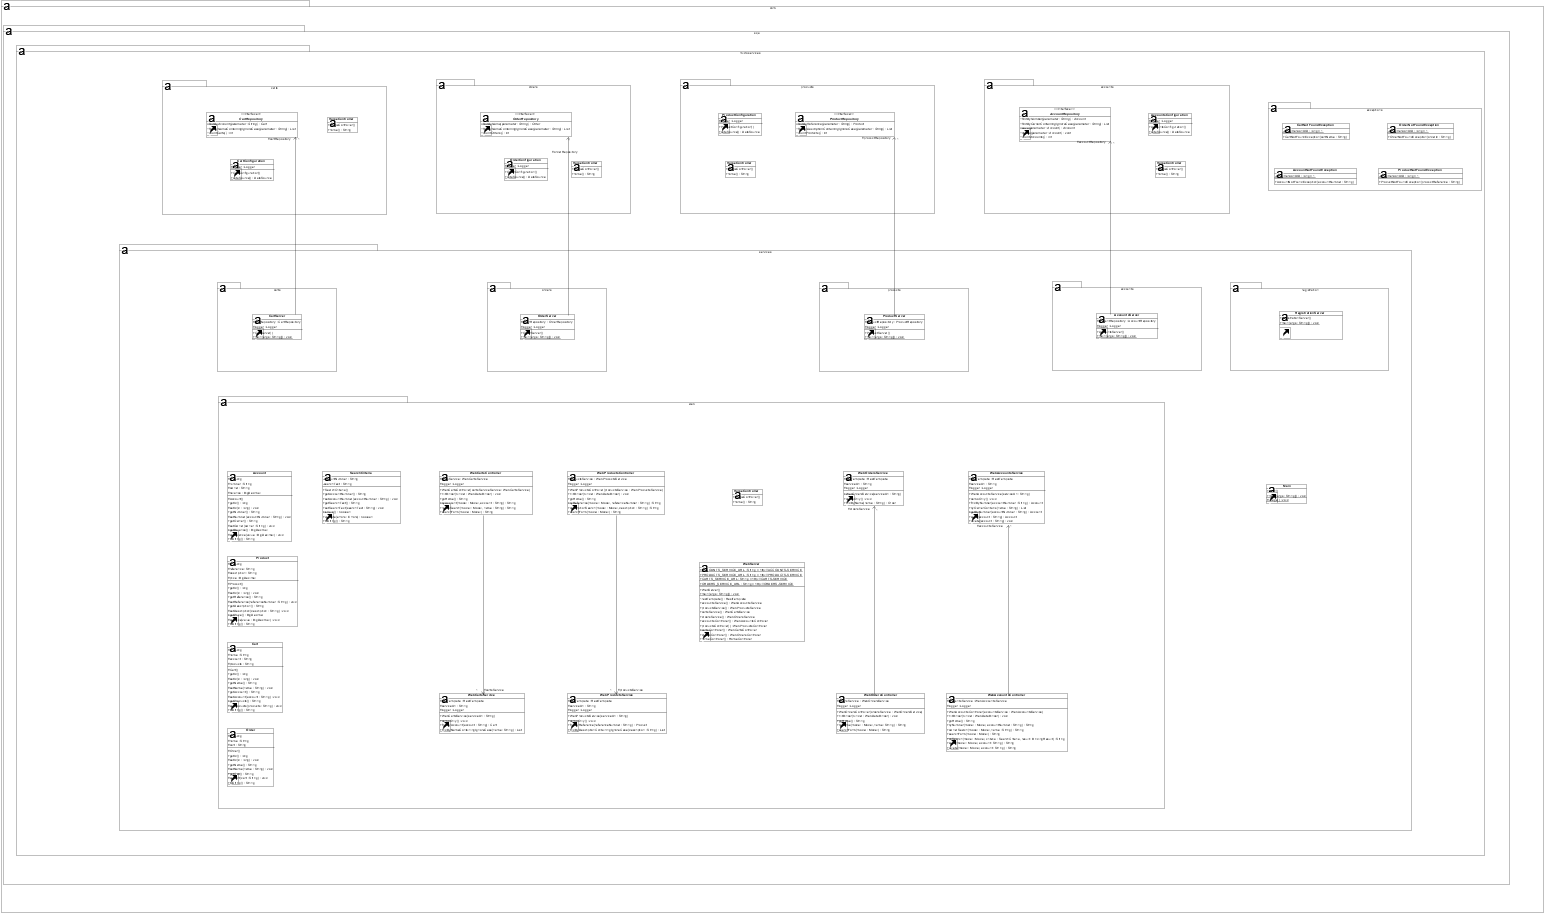
\includegraphics[width=\textwidth,height=\textheight,keepaspectratio]{Figures/ClassDiagram.png}
\decoRule
\caption[Class Diagram]{Application class diagram}
\label{fig:Class Diagram}
\end{figure}

\paragraph So at the end the feature files define requirements for both a service provider and a service consumer and that those services shall be independent between each other. In \ref{fig:Class Diagram} the four service packages are found at the top of the diagram (the right most package correspond to the Exceptions classes used by the services) which are Accounts service, Product service, Cart service and Order service. Here is where the data model and the provider REST API is configured. Registration service is configured within Spring and so no need a package here. Each one of these service classes has then a connection to the the server classes below, used for triggering each service and for exposing its REST API. The right most server package host the server class for the Registration service. 

\paragraph Below the server packages for the functional services, there is the Web server package where a consumer REST API for each one of the services is configured and exposed. Finally, the lonely class a the center right of the diagram is the Main class that will call one of the server classes depending on the incoming arguments ([accounts | product | cart | order | web | registration]).

%-----------------------------------------------------------------------------------------------------------------

\section{REST API}

The features described before define some requests to the services that are fulfilled with the following REST API.

\subsection{Producer API}

\subsubsection{Accounts}
\begin{itemize}
	\item \textit{/accounts/{number}}: search for an account by its account number.
	\item \textit{/accounts/owner/{name}}: search for an account by its account owner name.
	\item \textit{/accounts/save/{account}}: saves a new account.
	\item \textit{/accounts/delete/{account}}: deletes an existing account.
\end{itemize}

\subsubsection{Products}
\begin{itemize}
	\item \textit{/products/{reference}}: search for a product by its product reference.
	\item \textit{/products/description/{description}}: search for a product by its product description.
	\item \textit{/products/save/{product}}: saves a new product.
	\item \textit{/products/delete/{product}}: deletes an existing product.
\end{itemize}

\subsubsection{Carts}
\begin{itemize}
	\item \textit{/carts/{account}}: search for a cart by its associated account number.
	\item \textit{/carts/name/{name}}: search for a cart by its name.
	\item \textit{/carts/save/{cart}}: saves a new cart.
	\item \textit{/carts/delete/{cart}}: deletes an existing cart.
\end{itemize}

\subsubsection{Orders}
\begin{itemize}
	\item \textit{/orders/{name}}: search for an order by its order name.
	\item \textit{/orders/save/{order}}: saves a new order.
	\item \textit{/orders/delete/{order}}: deletes an existing order.
\end{itemize}


\subsection{Consumer API}

\subsubsection{Web}
Its API is just a mapping to the services consumer API defined below.

\subsubsection{Accounts}
Its API is just a mapping to the Accounts provider API defined above.

\subsubsection{Products}
Its API is just a mapping to the Products provider API defined above.

\subsubsection{Carts}
Its API is just a mapping to the Carts provider API defined above.

\subsubsection{Orders}
Its API is just a mapping to the Orders provider API defined above.

\subsubsection{Registration}
As this service is based in the Eureka project, its API is specified in the corresponding official documentation: 
\hyperref[]{\textcolor[rgb]{0,0,1}{https://github.com/Netflix/eureka/wiki/Eureka-REST-operations}}
Registration service API is not required directly by the features defined in this chapter but is used by the test steps that check connectivity with the Web server and by the ones that verify the availability requirements.


%-----------------------------------------------------------------------------------------------------------------